% Chapter 2

\chapter{Experimental Model} % Main chapter title
\label{Chapter3}

The first phase of this project was to design and select an appropriate 
experimental model. This was essential to gather the necessary data from the 
tested material. This data will be used to determine the design parameters 
that can help to characterize the material's mechanical behavior. \\

The experimental model I had the purpose of serving as a comparator for the experimental 
model II (see Section \ref{section:expmod2}). At the beginning of the project, the desired experimental 
model to be analyzed was the second experimental model, which was developed and designed by Yokohama National 
University (YNU). As this second experimental model was still undergoing some improvements and corrections, a similar 
experiment was designed which could fulfill the same purpose.

The chosen experimental characterization for the inverse finite element method for 
 the identification of material parameters for this project was indentation.
The goal of these experiments was to observe the mechanical behavior of a soft material under 
compression using a rounded indenter. The aim was to determine the material behavior and 
observe the response under an indentation larger than the indenter radius. Additionally, 
by performing the indentation tests, the obtained 
data helped for a more in-depth understanding of the material's mechanical behavior for the chosen 
use cases and the determination of the main assumptions for the material modeling.
The main advantage of indentation is the noninvasive feature, which will mostly 
become useful when a test sample should not be modified, e.g., an organ.\\

For both experimental setups, the specimen, which was tested, was made from a human skin gel.
The human skin gel material was a two-component ultra-soft urethane resin.
Polyurethane is widely used for biomedical applications, e.g., preparation of implants, wound dressings, artificial 
organs, and medical supplies. 

Polyurethane can also be used for simulating organ tissues, as it can be tailored to mimic 
and match the mechanical properties of the desired biological tissues \cite{Wang2012}.  Furthermore, polyurethane can be 
synthesized to have a wide range of stiffness, elasticity, viscoelasticity, and can also be prepared 
with complex shapes for medical research purposes \cite{Joseph2018}. \\

In this chapter, the different experimental models, which were used to evaluate the 
mechanical behavior of the ultra-soft polyurethane, will be 
described. In the first two subsections, will focus on the description and 
procedure of the experimental models, followed by explanation of the indentation test 
types. Consequently, an evaluation and analysis of the results will be provided and the 
main assumptions for the design of the material modeling will be defined. 
%The aim in this section is to provide a clear undertanding of the material's mechanical behavior, 
%and describe the first step for the inverse finite element method approach.
% Polyurethane can be easily processed by using 
%standard manufacturing, like %search reference
%here urethane resin avantages. and that it is expected that the material shows a 
\\ 

%----------------------------------------------------------------------------------

\section{Experimental Model I}
\label{section:expmod1}
    
\subsection*{Description of the Experimental Setup}

The first indentation test configuration was done by adapting a tensile and compression 
testing machine, model LTS - 500 NB from MinebeaMitsumi.Inc (Fig. \ref{fig:firstexperiment}). This 
machine possess a maximum load capacity of \SI{500}{\newton}, and test speeds of
\SIlist[per-mode = symbol]{10;20;30;50;75;100}{\milli \metre \per \minute}. To achieve an 
indentation testing configuration, a pin was attached to the movable crosshead holding grip, 
as shown in Fig \ref{fig:500loadcell}.
The indenter had a rounded head made of stainless steel with a
radius of $r_{i1} = \SI{3}{\milli \m}$ and a length of $l_{i1} = \SI{11}{\milli \m}$.

\begin{figure}%
    \centering
   \subfloat[\centering Indentation test configuration with a \SI{500}{\newton} load cell \label{fig:500loadcell}]{{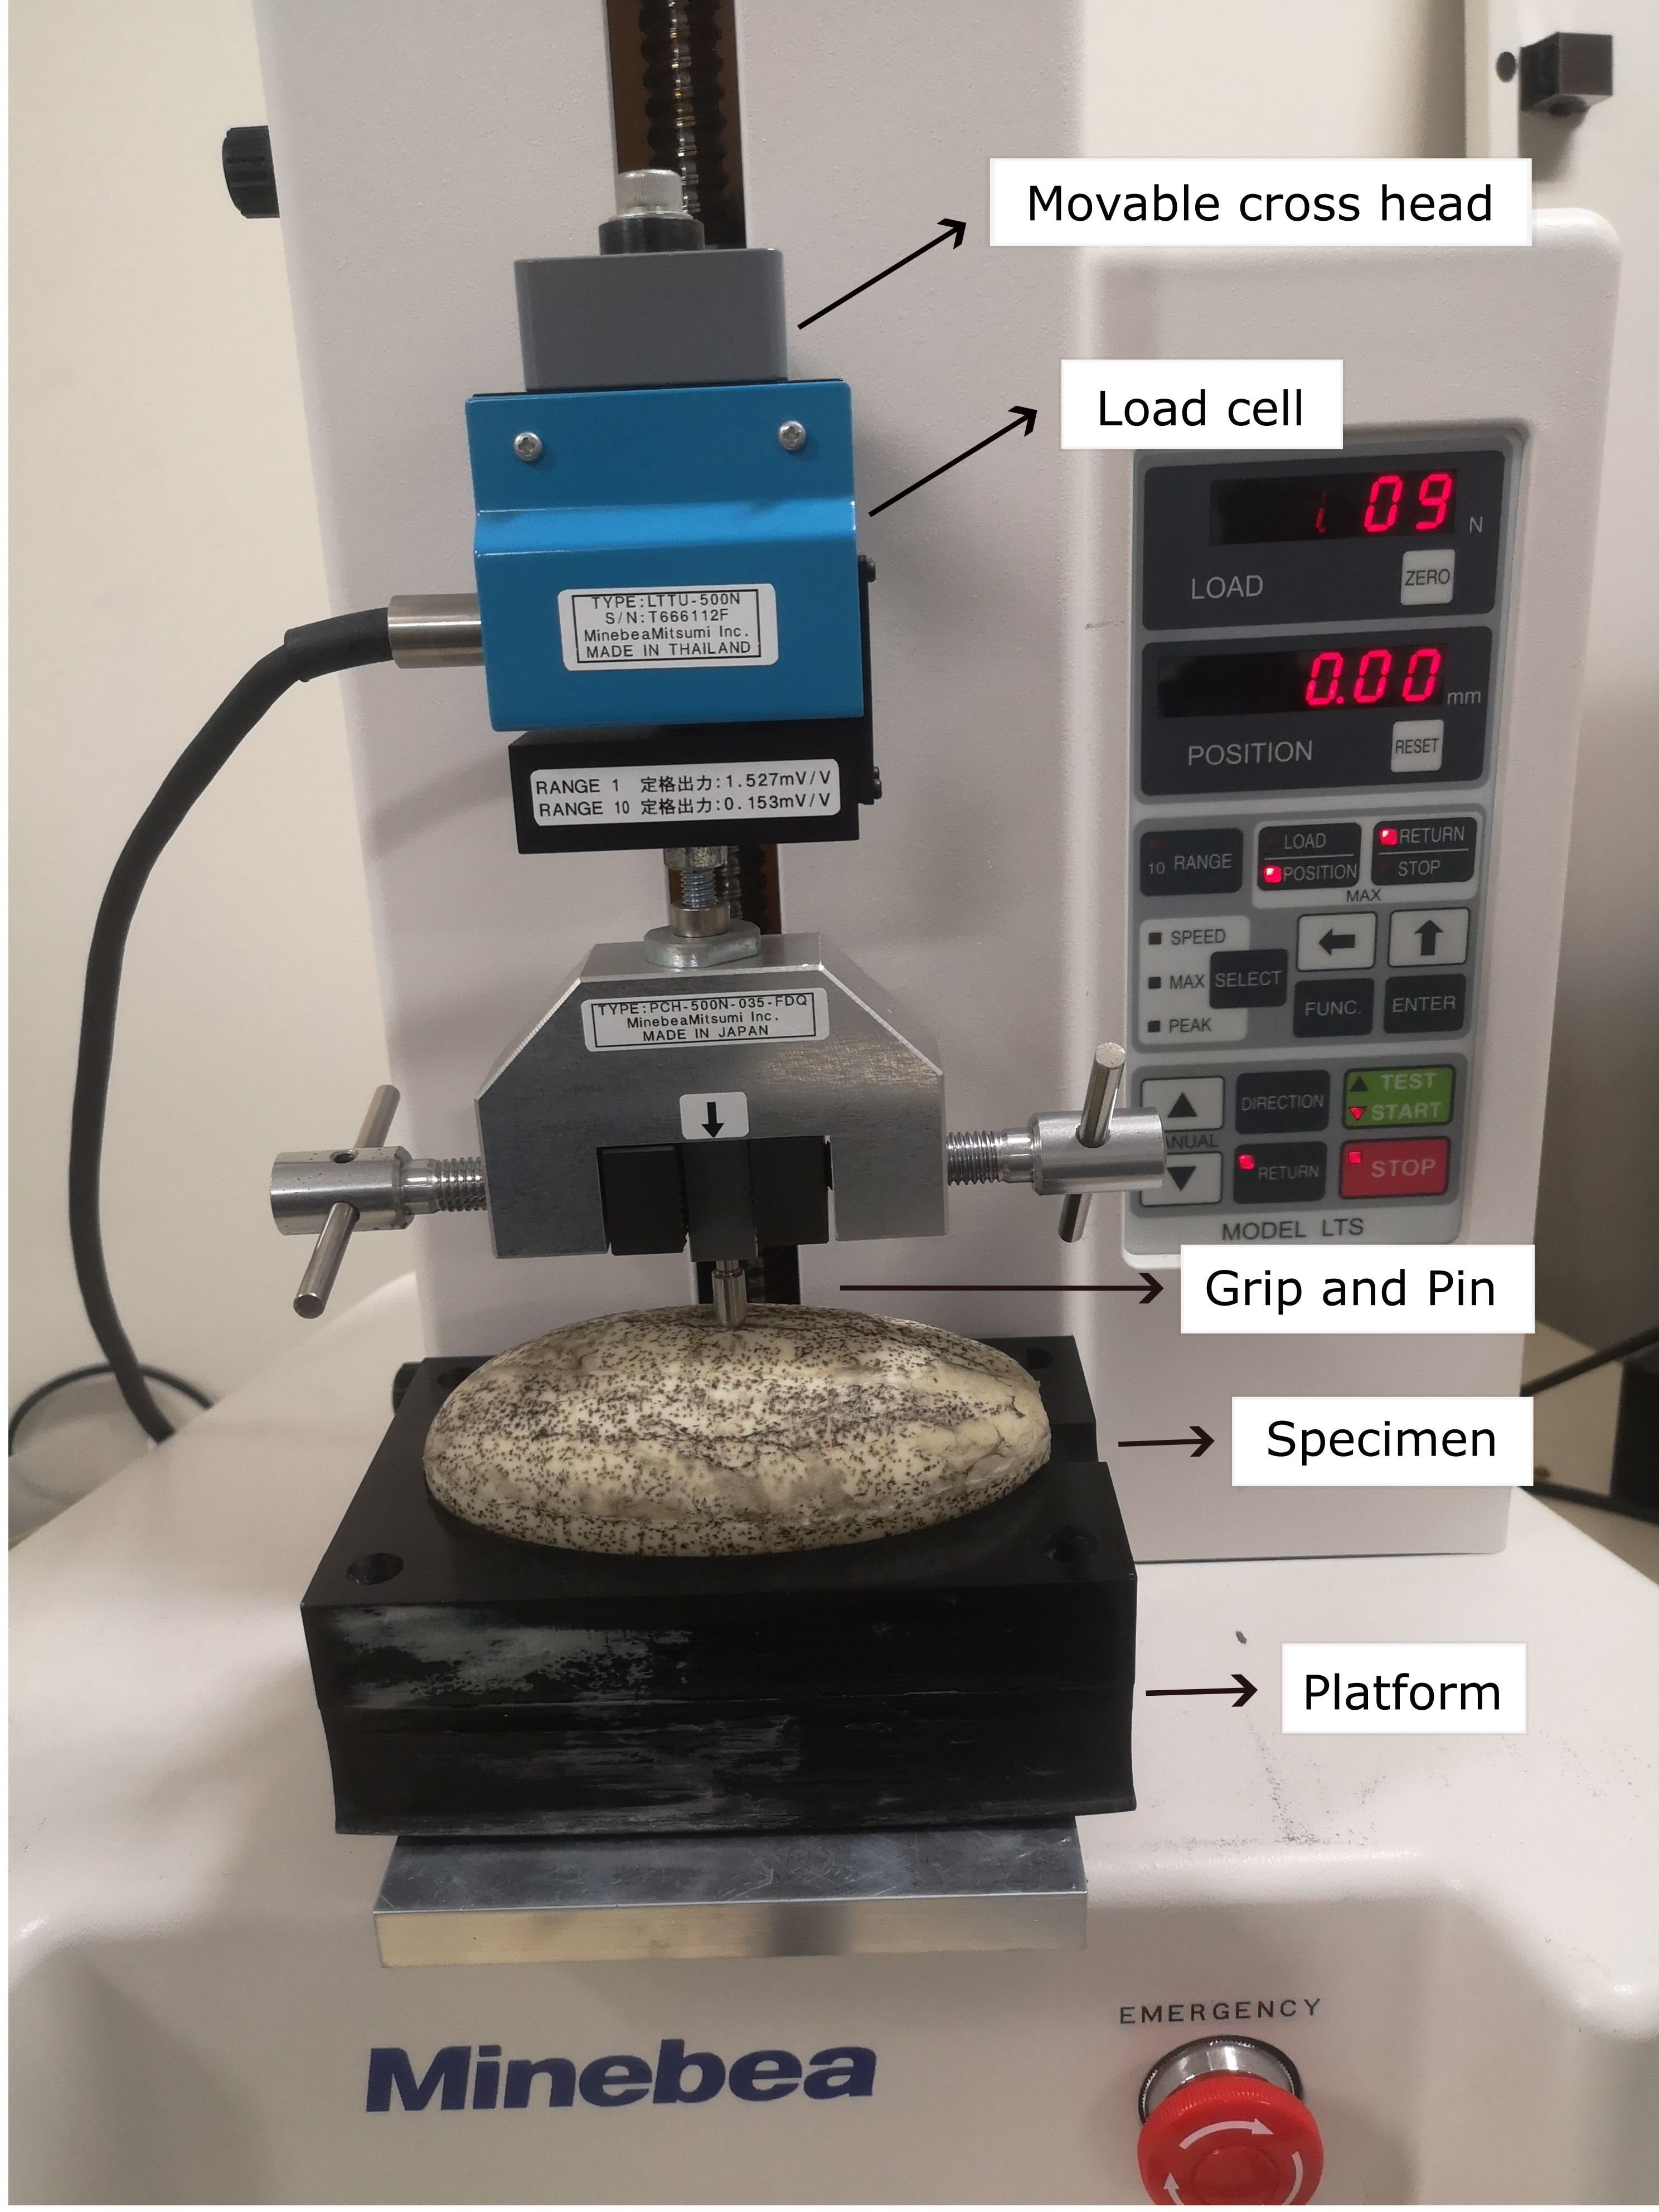
\includegraphics[width=6.5cm]{Images/Experiment/firstexperimentwithtext.png}}}%
   \qquad
   \subfloat[\centering Indentation test configuration with a \SI{10}{\newton} load cell \label{fig:10loadcell}]{{\includegraphics[width=6.5cm]{Images/Experiment/firstexpotherloadwithtext.png}}}%
   \caption{First experimental model: Tensile and compression machine with an indenter with a rounded head. Test Specimen made from ultra-soft polyurethane resin positioned on a fixed platform with a similar shape for constraint.}%
   \label{fig:firstexperiment}%
\end{figure}

The specimen possesses a ellipsoidal form with 
with a minor radius $r_1 = \SI{35}{\milli \m}$ and a major radius $r_2 = \SI{60}{\milli \m}$. 
This specimen geometry is supposed to simulate a kidney with an extracted tumor; therefore,
on the lower part of the specimen a half ellipsoid with a minor radius $r_{l1} = \SI{10}{\milli \m}$ 
and a major radius $r_{l2} = \SI{15}{\milli \m}$ was removed (Fig. \ref{fig:specimenhole}). 
The specimen was prepared by a YNU laboratory member, by 3D printing a mold with the wanted dimensions
 and a ellipsoidal shape, and filling it with liquid resin. 
 Additionally, it was left to cure for around \SI{30} hours. It is relevant to clarify, that this 
 sample had been created months before the development of this experimental setup and 
 had been utilized in other projects conducted from the laboratory.
This available specimen was positioned on a platform fixed to the base, which suited 
the ellipsoidal geometry for properly constraint. 

\begin{figure}%
    \centering
   \subfloat[\centering Specimen dimensions bottom view \label{fig:specimenunder}]{{\includegraphics[width=6.5cm]{Images/Experiment/specimenhole.png}}}%
   \qquad
   \subfloat[\centering Specimen side view \label{fig:specimenside}]{{\includegraphics[width=6.5cm]{Images/Experiment/specimenholeside.png}}}%
   \caption{First experimental model: Specimen dimensions made from ultra-soft polyurethane resin for indentation test.}%
   \label{fig:specimenhole}%
\end{figure}

\subsection*{Procedure for Conducting the Experiment}
For the indentation test after placing the specimen on the platform,
the indenter was positioned slightly on the surface of the point of interest. 
The test was conducted with a room temperature of approximately \SI{22}{\degreeCelsius}
To perform the test the indenter was then lowered onto the surface of the specimen
at a velocity of \SI[per-mode = symbol]{10}{\milli \m\per \minute}.
The indentation depth was controlled by limiting the maximum depth, and the 
test stopped once the inserted depth was reached. The indenter returned to its 
original position after reaching the maximum depth with a rate of 
\SI[per-mode = symbol]{100}{\milli \m\per \minute}. Due to the material properties,
the specimen returned to its original shape.
The result of the indentation test was a load-displacement data,
which was recorded with a sampling rate of \SI{63}{\hertz} using a load 
cell of \SI{\pm 500}{\newton} and a encoder to measure the displacement.

The measurement accuracy according to the specification of the machine, has 
a relative reading error of \SI{1.0}{\percent}. The indentation test 
was repeated five times on the same sample to ensure and observe 
reliability and repeatability. Furthermore, the raw data collected from the test 
was processed and analyzed using Excel.\\

During the initial indentation test using the \SI{500}{\newton} load cell, 
the collected experimental data showed noise that could affect the accuracy 
and reliability of the results. The noise was likely caused by sensitivity 
of the lead cell. The ultra-soft polyurethane material showed force readings, which 
were near the lower limit of the load cell's range, which adding any other external factors, 
results in noisy measurements. To address this issue, a load cell of \SI{10}{\newton}
was installed (Fig. \ref{fig:10loadcell}). This change improved the quality of 
the measurements and reduced the noise in the data. The change to the load cell had some 
implication to the experimental setup, such as removing the holding grip, and designing 
a part which could connect the indenter with the new load cell. In addition to changing 
the load cell, a simple filtering method was used to improve the experimental data. After 
applying the filter, the noise in the data was reduced, resulting in more smoother 
force reaction readings. 

The applications of the combinations helped to improved the quality and acuracy 
of the data and gave important information about possible measurement errors to 
take into consideration for of the experimental model 
designed by YNU. At last, The filtered data was used for subsequent analysis and 
interpretation for the inverse finite element method approach for the material parameter 
identification.

%iii.	Analysis of different platforms? maybe dont because not enough fotos or info

%----------------------------------------------------------------------------------
\section{Experimental Model II}
\label{section:expmod2}

The second experimental model was developed and designed by Yuta Mori, a 
member of the Yamada Laboratory from the Mechanical Engineering department of 
 Yokohama National University. 
The main aim for this experimental method was to be able to identify the physical 
properties of organs in a state that closely resembles the in vivo environment.
Additionally, this model seeked two achieve two objectives: firstly, to develop a 
loading system to acquire the data required for an inverse analysis, and secondly, 
to establish a measurement process in case of a total nephrectomy \cite{Mori2022}. 

Furthermore, for the present experimental setup a new sample was prepared using 
the same material as the previous one, i.e., human skin gel made from ultra-soft 
polyurethane resin, and following the same 
manufacturing processs as decribe in Section \ref{section:expmod1}. 
%evtl. speak about ehical use of the experimental model : To ensure the ethical use of the experimental model and data provided by the other master student, I obtained permission from them to use their data in my research. Additionally, I made sure that any ethical considerations related to the data, such as informed consent from participants or privacy concerns, 
%had been appropriately addressed in the original study. As an extra precaution, I also ensured that any identifiable information about the participants had been removed from the data provided by the other master student before incorporating it into my own research. By taking these steps, I ensured that the data was used in a responsible and ethical manner, and that the original research was respected and properly attributed

The resulting data from the experimental model served for the basis of the material 
parameter identification for the inverse finite element method approach.
The processed data obtained from this experimental model assisted in the calibration 
and assessment of the design parameters was employ in the validation for the 
computational model. 

\subsection*{Description and Procedure of the Experimental Setup}
%This article discusses the development of a method to identify the mechanical properties of organs after extraction. 
%The study aims to identify the physical properties of organs immediately after removal to simulate in vivo environments. 
%The study constructs a loading system to acquire data for inverse analysis and establish a measurement process to conduct
% multi-point loading experiments and simultaneously measure the indentation, reaction force, and overall deformation. 
% The study uses a 6-axis force sensor, a laser displacement transducer, and 3D cameras to measure reaction forces, 
% organ deformation, and organ shape. The experimental results show that the method can measure organ mechanical 
% properties and provide data for simulators.

In this experimental model the indentation loading system, which gathers data of the indentation 
depth, reaction force and general deformation. 
The experimental device consists of an 6-axis force sensor, a laser displacement transducer,
 and 3D cameras placed in four directions to obtain the point cloud data based on the 
 coordinate system of each camera. Fig.\ref{fig:secondexperiment} shows the setup of the 
 experiment. For our project, the 6-axis force sensor and the laser displacement were mainly used.
The loading system is operated by specifiying de movement of the loading rod in advance, and the 
indentation is performed in the direction normal to the contact surface to prevent slippage (Fig. \ref{fig:loadingdiag}).\\

 \begin{figure}%
    \centering
   \subfloat[\centering Indentation test configuration front view \label{fig:frontexp2}]{{\includegraphics[width=6.5cm]{Images/Experiment/secondexp1}}}%
   \qquad
   \subfloat[\centering Indentation test configuration top view \label{fig:topexp2}]{{\includegraphics[width=6.5cm]{Images/Experiment/secondexp2.jpg}}}%
   \caption{YNU experimental model: 6-axis sensor Test Specimen made from ultra-soft polyurethane resin positioned on a fixed platform with a similar shape for constraint.}%
   \label{fig:secondexperiment}%
\end{figure}

\begin{figure}%
    \centering
   \quad
   \includegraphics[width=6.5cm]{Images/Experiment/Loadingdiagram.png}%
   \caption{YNU experimental model: Loading diagram showing initial position of the indenter in normal position \cite{Mori2022}.}%
   \label{fig:loadingdiag}%
\end{figure}

The specimen, same as in the first experimental model (Section \ref{section:expmod1}),
 possessed the same dimensions, a minor radius $r_1 = \SI{35}{\milli \m}$ and a major 
 radius $r_2 = \SI{60}{\milli \m}$, and was
made from ultra-soft polyurethane resin. Consequently, the platform is also 
bowl-shaped. For this experiment, the platform base was made from transparent 
acrylic resin to record the contact status of the bottom surface \cite{Mori2022}. 
The maximum load capacity of the load cell is \SI{200}{\newton} and a theoretical 
force resolution of \SI{0.001}{\newton}. In addition, the resolution of the 
laser displacement sensor is \SI{0.05}{\milli \m}.
The indenter is sphere-shaped with a radius of $r_{i2} = \SI{3}{\milli \m}$ and
was made from ruby with the following specifications; 
a Young's Modulus of $E_{i2} = \SI{440}{\giga \pascal}$ and a Poisson's ratio of 
$\nu_{i2} = \SI{0.3}{\milli \m}$.\\

The indentation test was conducted under room temperature conditions. Also, 
the sample was placed on acrylic platform and the indenter was 
lowered at constant velocity of \SI[per-mode = symbol]{30}{\milli \m\per \minute}. 
The experiments were conducted for each loading point five times on the same sample, 
and the average of the results were calculated.

Furthermore, to minimize the friction during the indentation processs, the indenter 
and the loading surface on the specimen were covered with a thin layer of lotion. 
This was done due to inaccuracies and step-like data shown in the measurements. Therefore, to reduce 
this measurement error, the application of lubricant was employed, ensuring a 
smoother and more controlled indentation process. Finally, the data 
was also processed and assessed using Excel.

\subsection*{Analysis and Comparison of Experimental Techniques}

%write about the advantage and comparison
The second experimental model offers some advantages over the first model. 
Firstly, it enables not only the measurement of the total force reaction, but also the analysis 
of the force reaction components $F_x$, $F_y$ and $F_z$. This allows for a better 
understanding of the material's mechanical behavior, as it allows the identification 
of a specific contribution of the force components and it contributes to identify other 
mechanisms such as viscoelasticity, plasticity, and creep. 
In addition, the second model allowed for the measurement of the deformation in other 
points near the tested loading point. This provides additional information of the 
material parameters, as it facilitates the characterization of the deformation behavior beyond the 
direct vicinity of the indentation point. Furthermore, only this test configuration makes 
use of a lubricant, as this experimental setup could show some inaccuracies in the first data sample.

In contrast, the first experimental model only measures the total force reaction 
against the indentation depth, without providing any information about the contribution 
of each component. While the first model allows the data 
gathering in simpler and more straightforward way, it may not capture 
the whole complexity of the material.

%----------------------------------------------------------------------------------
\section{Experimental Tests Description}

\subsection{Middle Point}
\label{subsection:midpoint}
The first use case for the indentation test was performed at the midpoint 
of the major and minor axis of the ellipsoid (Fig. \ref{fig:midpoint}). This point was selected 
to ensure that the indentation was normal to the surface, thereby avoiding 
the influence of potential shear forces which could influence the 
measurements.

\begin{figure}%
    \centering
   \quad
   \includegraphics[width=6.5cm]{Images/Experiment/specimenmidp.png}%
   \caption{Middle test point: Loading point on the top surface of the specimen.}%
   \label{fig:midpoint}%
\end{figure}

Additionally, the first indentation depth was chosen arbitriarily, for the first 
experimental model was $h_{I} = \SI{3.8}{\milli \m}$, and for the second 
experimental model was $h_{II} = \SI{4}{\milli \m}$. This depth was considered 
to be an appropiate compromise that would allow to capture the nonlinear 
behavior of the material, while also remaining a simple use case to 
reproduce in a computational model in ANSYS.\\

As the main objective is to find a path, which lets identify the material 
 parameters, the most basic use case was selected and from this point 
the complexity was gradually built on. Through this approach, it was possible 
to establish a solid foundation for the subsequent experiments and data analysis.



\subsection{Load-Unloading}
\label{subsection:loadunload}
Building on the previous test point (Fig. \ref{fig:midpoint}), an indentation
 test was condunted on the same point, with the an indentation depth of 
 \SI{4}{\milli \m}, but this time in a loading-unloading case.

The first experimental model setup, as describe in Section \ref{section:expmod1},
was unable to measure the displacement and force reaction during the unloading 
of the specimen. As a result, certain modifications were made to the experimental 
setup. Due to time constraints, the modification of experimental model I 
was also executed by laboratory members Mori Yuta in YNU.
To capture the displacement and force reaction during the unloading, an 
displacement transducer was equipped to the tensile and compression machine 
as shown in Figure \ref{fig:unloadingexp1}.

\begin{figure}%
    \centering
   \quad
   \includegraphics[width=6.5cm]{Images/Experiment/unloading.png}%
   \caption{Load-Unload Case: Experimental model I with modified configuration setup, on top of the movable crosshead a displacement transducer was equipped to capture unloading data.}%
   \label{fig:unloadingexp1}%
\end{figure}
 
The aim of this use case, was the observation of a possible hysteresis
behavior, as well as to investigate the viscoelastic properties of the material.
The load-unload test was performed at six different loading speeds, namely, 
\SIlist[per-mode = symbol]{10;20;30;50;75;100}{\milli \metre \per \minute} on the 
same specimen.
Each speed configuration was reapeated five times, and te results were average to 
reduce the effects of experimental variability.\\

The load-unload case helped to determine whether complex material behavior such as 
viscoelasticity, could be neglected for the computational model of the middle point test.
The result of this experiment were used to make this decision, which has important 
implications for the simplification of the computational model and its accuracy and reliability.
%Escribir sobre experimental model 2?

\subsection{Nearby Point}
\label{subsection:nearbypoint}
%DataSummary230210Yuta
In addition to the indentation performed on the middle point of the surface, further 
indentations were conducted on nearby points. From these indentation tests, force-displacement 
curves were recorded. For each indentation the same experiment configuration, 
e.g., indentation depth and indentation 
speed, was employed as described in Sections \ref{section:expmod1} and \ref{section:expmod2}.

For the first experimental model, only one nearby point located $p_{I1} = \SI{5}{\milli \m}$ 
to the right of the middle point was selected as shown in Figure \ref{fig:nbdiagexp1}.

\begin{figure}%
    \centering
   \subfloat[\centering Nearby point location for Experimental model I \label{fig:nbdiagexp1}]{{\includegraphics[width=6.5cm]{Images/Experiment/nbexp1.png}}}%
   \qquad
   \subfloat[\centering Nearby points location for Experimental model II \label{fig:nbdiagexp2}]{{\includegraphics[width=6.5cm]{Images/Experiment/nbexp2.png}}}%
   \caption{Nearby test point: Loading points for each experimental model to analyze shear stresses and to vbe employed for the validation of the computation models.}%
   \label{fig:nbexp}%
\end{figure}

For the second experimental model, three additional nearby points were tested. 
These points were located at distance of $p_{II1} = \SI{20}{\milli \m}$ to the 
right, $p_{II2} = \SI{20}{\milli \m}$ downwards, and a third point $p_{II3} = \SI{28.3}{\milli \m}$ 
diagonally from the middle point forming a square (Fig. \ref{fig:nbdiagexp2}). \\

The objective of these testing points was to gain a deeper understanding of the effect of 
the shear stresses on the indentation response. Furthermore, 
the results of these points allowed for the validation of the 
computational model and the selected material model.



%For example, in a viscoelastic material, the initial loading response may be dominated by elastic behavior, followed by a time-dependent relaxation behavior as the material responds to the applied load. In contrast, a plastic material may exhibit a more gradual force response with continued loading, indicating the progressive deformation and flow of the material.
%By analyzing the force components during an indentation experiment, it is possible to separate out the contributions of different deformation mechanisms and gain a more nuanced understanding of the material's mechanical behavior. This can be achieved through various analytical techniques such as numerical simulations or mathematical models that take into account the material's constitutive behavior and mechanical properties.
%Overall, the observation of force components in an indentation experiment can provide important information about the underlying mechanisms contributing to the material's deformation behavior, which can be useful in a variety of engineering and scientific applications.

%----------------------------------------------------------------------------------
\section{Analysis and Overview of the Data and Results}
\label{section:expresult}
%Summary of the experimental models
%Results of the indentation test
%Discussion of the results
%conclusion

In this section, the results of the experimental models described in the previous 
sections will be presented and analyzed. The objective is to understand the behavior 
of this ultra-soft polyurethane material under indentation and establish the first 
assumptions for the development of the computational model, as well as the material model.
The section will start with a brief summary of the tests, followed by the analysis of the 
force-stroke curves gathered throughout the experiments.

The experimental model I served mainly as a comparator and a quick way to gain an idea of the 
mechanical behavior under indentation, for this model three differents use cases were measured. 
An indentation in the middle point of the surface with and indentation depth of $h_{I} = \SI{3.8}{\milli \m}$. 
Subsequently, the load-unload case was observed under an indentation depth of  $h_{I2} = \SI{4}{\milli \m}$, and 
with six different speeds ranging from \SI[per-mode = symbol]{10}{\milli \m\per \minute} to 
\SI[per-mode = symbol]{100}{\milli \m\per \minute}. 
Finally, a nearby point was selected near the middle point, $p_{I1} = \SI{5}{\milli \m}$ to the right,
 to use it as a validation point for the selected material model. 

A similar process was followed for the experimental model II, the middle point indentation was 
performed with an indentation depth of $h_{II} = \SI{4}{\milli \m}$ and a indentation 
speed of \SI[per-mode = symbol]{30}{\milli \m\per \minute}, where the force components 
could be observed. Similarly, the load-unload scenario was tested under the same conditions, and three 
nearby points were measured.

%----------------------------------------------------------------------------------
\subsection{Middle Point}
\label{subsection:midpointresult}
%EXPII:20230301_Progress_Report_'3_4mm/Average_Force-Stroke
The results of the indentation test at the middle point for both experimental showed a clear 
nonlinear behavior.  It is assumed that this material 
possess a elastic-plastic behavior, which in a typical load-displacement curves has four known stages \cite{Goharian2017}:

\begin{enumerate}
    \item Nonlinear elastic (self-adjusting): In this stage, the material adjusts itself to the loading conditions, and the deformation is elastic and reversible.
    \item Linear elastic: The material is bearing the external load in this stage, the deformation is still elastic and reversible 
    \item Nonlinear plastic (failing): With the increase of the external load, the material reaches its yield point and undergoes permament deformation
    \item Failure: The material fails leading to permanent damage.
\end{enumerate}


Figure \ref{fig:midpointgraph} shows the results of the two indentations at the middle point 
 of the specimen surface.
The load-displacement curves showed nearly identical material behavior for both 
experimental configurations. This use case demonstrate the nonlinear-elastic behavior of the material, 
as there was no evidence of a yield point or plastic behavior. 
Both curves began at zero, and the force increased gradually with increasing,
resulting in a slightly concave shape. 

Figure \ref{fig:mpIexp} displays all the measurements points obtained from experimental model I and its 
polynomial approximation. This approximation was used for the subsequent steps of the iFEM approach. The 
maximum total force for experimental model I at a maximun indentation depth of 
$u_{I_{MP}} = \SI{3.8}{\milli \m}$ was $F_{I_{MP}} = \SI{0.4218}{\newton}$. For experimental 
model II, at an indentation depth of 
$u_{II_{MP}} = \SI{4}{\milli \m}$, the maximum forces for each component were
 $F_{Z_{II,MP}} = \SI{0.546}{\newton}$, $F_{Y_{II,MP}} = \SI{0.0124}{\newton}$, and $F_{X_{II,MP}} = \SI{0.0093}{\newton}$.\\

\begin{figure}%
    \centering
   \subfloat[\centering Experimental model I: Total force reaction - indentation depth graph \label{fig:mpIexp}]{{
        \begin{tikzpicture}[scale=0.76]
            \begin{axis}[
                xmax=4.2,xmin=0,
                ymin= 0,ymax=0.6,
                ytick={0,0.1,0.2,...,0.6},
                xlabel={Displacement $u [mm]$},
                ylabel={Force reaction $F_{I_{MP}}[N]$},
                grid = major,
                legend pos= north west]
                \addplot[gray,only marks, mark = x, opacity=0.2] table[x = Def, y = $Force$] {Table/Middle Point/MPI38all.dat};
                \addplot+[color=blue, smooth, very thick, no markers] table [y=$Force$, x=Def]{Table/Middle Point/MPI38mm.dat};
                \legend{Measurement, Total force reaction,test}
        \end{axis}
        \end{tikzpicture}}}%
   \qquad
   \subfloat[\centering Experimental model II: Force reaction components - indentation depth graph \label{fig:mpIIexp}]{{
    \begin{tikzpicture}[scale=0.76]
        \begin{axis}[
            xmax=4.2,xmin=0,
            ymin= 0,ymax=0.6,
            ytick={0,0.1,0.2,...,0.6},
            xlabel={Displacement $u [mm]$},
            ylabel={Force reaction $F_{II_{MP}} [N]$},
            grid = major,
            legend pos= north west]
            \addplot+[smooth, no markers, thick] table [y=$F_z$, x=Def]{Table/Middle Point/MPII4mm.dat};
            \addplot+[smooth, no markers, thick] table [y=$F_y$, x=Def]{Table/Middle Point/MPII4mm.dat};
            \addplot+[smooth, no markers, thick] table [y=$F_x$, x=Def]{Table/Middle Point/MPII4mm.dat};
            \legend{$F_z$,$F_y$,$F_x$}
        \end{axis}
    \end{tikzpicture}}}%
   \caption{Load-displacement curve experimental data for Middle Point use case for both experimental models.}%
   \label{fig:midpointgraph}%
\end{figure}

\begin{figure}%
    \centering
   \quad
    \begin{tikzpicture}[scale=1]
        \begin{axis}[
            xmax=4.2,xmin=0,
            ymin= 0,ymax=0.6,
            ytick={0,0.1,0.2,...,0.6},
            xlabel={Displacement $u [mm]$},
            ylabel={Force reaction $F_{MP} [N]$},
            grid = major,
            legend pos= north west]
            \addplot+[smooth, no markers, thick] table [y=$Force$, x=Def]{Table/Middle Point/MPI38mm.dat};
            \addplot+[smooth, no markers, thick] table [y=$Force$, x=Def]{Table/Middle Point/MPII4mmtotalap.dat};
            \legend{Experiment I,Experiment II}
        \end{axis}
    \end{tikzpicture}%
   \caption{Total Force Reaction-Displacement curve: Comparison between experimental data for Middle Point use case from both models.}%
   \label{fig:midpointexpIvsexpII}%
\end{figure}

From load-displacement curve of experimental model II (Fig. \ref{fig:mpIIexp}) it was evident that the
force reactions in the X and Y directions could be disregard, as these were considerably lower than
the force reaction in Z direction. Therefore, the focus in further analysis was mainly 
on the force reaction in Z direction. Additionally, this case revealed that shear stresses were minimal, 
which is consistent with the purpose on performing the indentation with the least influence of external factors.\\

Figure \ref{fig:midpointexpIvsexpII}, shows that the load-displacement curve
of experimental model I has a similar initial behavior to that of experimental model II.
However, as the indentation depth increases, the curve of experimental model I is positioned 
lower than that of the second model. One possible explanation for this difference could be the effect of aging 
on the material properties of the specimen used in the first model. Since the specimen used in this 
configuration was manufactured months before (Section \ref{section:expmod1}), it is possible that the aging 
had led to a decrease in its mechanical properties, resulting in a lower resistance to deformation
and therefore, lower stiffness than the newly manufactured sample.
Another possible explanation could be the presence of external factors during the conduction of 
the experiments or the configuration of these. Nevertheless, as the main purpose of this Middle Point 
use case was to minimize the influence of these factors, this explanation seems less probable.

%the difference between a and b graph can also be the that one sample is older as the other
%conclusion and limitation of MP:to appreciate a all the aspects of the material behaviour would be important to perform higher indentation 
%----------------------------------------------------------------------------------
\subsection{Load-Unloading}
\label{subsection:loadunloadresult}
%EXPII:20230203_Datasummary_4mmindentation/Average_Force-Stroke_0226
%EXPI:20221025_DataSharing_pptdocument/processeddata
Following the Middle Point use case, in addition to the loading data, the unloading was 
also captured for both experiments as explained in Section \ref{subsection:loadunload}.
Figure \ref{fig:loadunloadgraph} shows the load-displacement curve for experimental model 
I and next to it experimental model II. Both results exhibited during the unloading some 
degree of hysteresis, as there was a sligth difference in the force reaction measured.
However, the material displayed good elastic behavior, as it returned to its 
original shape once the indenter was removed.\\

%Different Load Unload
\begin{figure}%
    \centering
   \subfloat[\centering Experimental model I: Total force reaction - indentation depth graph \label{fig:luIexp}]{{
        \begin{tikzpicture}[scale=0.75]
            \begin{axis}[
                xmax=4.2,xmin=0,
                ymin= 0,ymax=0.6,
                ytick={0,0.1,0.2,...,0.6},
                xlabel={Displacement $u [mm]$},
                ylabel={Force reaction $F_{I_{LU}} [N]$},
                grid = major,
                legend pos= north west]
                \addplot+[smooth, no markers, thick] table [y=$Force$, x=Def]{Table/Loadunload/LI4mm.dat};
                \addplot+[smooth, no markers, thick] table [y=$Force$, x=Def]{Table/Loadunload/UI4mm.dat};
                \legend{Load I, Unload I}
            \end{axis}
        \end{tikzpicture}}}%
   \qquad
   \subfloat[\centering Experimental model II: Force reaction components - indentation depth graph \label{fig:luIIexp}]{{
    \begin{tikzpicture}[scale=0.75]
        \begin{axis}[
            xmax=4.2,xmin=0,
            ymin= 0,ymax=0.6,
            ytick={0,0.1,0.2,...,0.6},
            xlabel={Displacement $u [mm]$},
            ylabel={Force reaction $F_{II_{LU}} [N]$},
            grid = major,
            legend pos= north west]
            \addplot+[smooth, no markers, thick] table [y=$Force$, x=Def]{Table/Loadunload/LII4mm.dat};
            \addplot+[smooth, no markers, thick] table [y=$Force$, x=Def]{Table/Loadunload/UII4mm.dat};
            \legend{Load II, Unload II}
        \end{axis}
    \end{tikzpicture}}}%
   \caption{Load-displacement curve experimental data for Load-Unload use case for both experimental models.}%
   \label{fig:loadunloadgraph}%
\end{figure}

The hysteresis displayed for both configurations could have occured due to several reasons, such 
as viscoelastic behavior of the material, or external factors, like friction 
between the indenter and the specimen, surface roughness of the indenter, test configuration, and so on.
To examine closer the main reason for the hysteresis, only with first experimental setup,
a series of indentations tests were performed with different speeds.

Figure \ref{fig:ludifspeed} shows the result of the load-unload indentation tests from the lowest to 
highest value for the indentation speed. It could be observed, 
that the curves exhibit a similar material behavior. A slight 
increase in the hysteresis was observed when the indentation 
speed was increased. Specifically, during the loading, the 
force reaction were slightly higher as the speed and indentation depth increased.
During the unloading, the only notable difference was observed with 
\SI[per-mode = symbol]{100}{\milli \m\per \minute}, where the unloading curve
had the lowest values.\\

%Different Speeds Graph
\begin{figure}[htbp]
    \centering

    \begin{subfigure}[b]{0.45\textwidth}
    \centering
    \begin{tikzpicture}[scale=0.78]
        \begin{axis}[
            xmax=4.2,xmin=0,
            ymin= 0,ymax=0.6,
            ytick={0,0.1,0.2,...,0.6},
            xlabel={Displacement $u [mm]$},
            ylabel={Force reaction $F_{I_{LU}} [N]$},
            grid = major,
            legend pos= north west]
            \addplot+[smooth, no markers, thick] table [y=$Force$, x=Def]{Table/Loadunload/Speed/L10.dat};
            \addplot+[smooth, no markers, thick] table [y=$Force$, x=Def]{Table/Loadunload/Speed/U10.dat};
            \legend{Load, Unload}
        \end{axis}
    \end{tikzpicture}
    \caption{\SI[per-mode = symbol]{10}{\milli \m\per \minute}}
    \end{subfigure}
    \hspace{0.3cm}
    \begin{subfigure}[b]{0.45\textwidth}
    \centering
    \begin{tikzpicture}[scale=0.78]
        \begin{axis}[
            xmax=4.2,xmin=0,
            ymin= 0,ymax=0.6,
            ytick={0,0.1,0.2,...,0.6},
            xlabel={Displacement $u [mm]$},
            ylabel={Force reaction $F_{I_{LU}} [N]$},
            grid = major,
            legend pos= north west]
            \addplot+[smooth, no markers, thick] table [y=$Force$, x=Def]{Table/Loadunload/Speed/L20.dat};
            \addplot+[smooth, no markers, thick] table [y=$Force$, x=Def]{Table/Loadunload/Speed/U20.dat};
            \legend{Load, Unload}
        \end{axis}
    \end{tikzpicture}
    \caption{\SI[per-mode = symbol]{20}{\milli \m\per \minute}}
    \end{subfigure}
    \vspace{0.5cm}
    \begin{subfigure}[b]{0.45\textwidth}
    \centering
    \begin{tikzpicture}[scale=0.78]
        \begin{axis}[
            xmax=4.2,xmin=0,
            ymin= 0,ymax=0.6,
            ytick={0,0.1,0.2,...,0.6},
            xlabel={Displacement $u [mm]$},
            ylabel={Force reaction $F_{I_{LU}} [N]$},
            grid = major,
            legend pos= north west]
            \addplot+[smooth, no markers, thick] table [y=$Force$, x=Def]{Table/Loadunload/Speed/L30.dat};
            \addplot+[smooth, no markers, thick] table [y=$Force$, x=Def]{Table/Loadunload/Speed/U30.dat};
            \legend{Load, Unload}
        \end{axis}
    \end{tikzpicture}
    \caption{\SI[per-mode = symbol]{30}{\milli \m\per \minute}}
    \end{subfigure}  
    \hspace{0.3cm}
    \begin{subfigure}[b]{0.45\textwidth}
    \centering
    \begin{tikzpicture}[scale=0.78]
        \begin{axis}[
            xmax=4.2,xmin=0,
            ymin= 0,ymax=0.6,
            ytick={0,0.1,0.2,...,0.6},
            xlabel={Displacement $u [mm]$},
            ylabel={Force reaction $F_{I_{LU}} [N]$},
            grid = major,
            legend pos= north west]
            \addplot+[smooth, no markers, thick] table [y=$Force$, x=Def]{Table/Loadunload/Speed/L50.dat};
            \addplot+[smooth, no markers, thick] table [y=$Force$, x=Def]{Table/Loadunload/Speed/U50.dat};
            \legend{Load, Unload}
        \end{axis}
    \end{tikzpicture}
    \caption{\SI[per-mode = symbol]{50}{\milli \m\per \minute}}
    \end{subfigure}
    \vspace{0.5cm}
    \begin{subfigure}[b]{0.45\textwidth}
    \centering
    \begin{tikzpicture}[scale=0.78]
        \begin{axis}[
            xmax=4.2,xmin=0,
            ymin= 0,ymax=0.6,
            ytick={0,0.1,0.2,...,0.6},
            xlabel={Displacement $u [mm]$},
            ylabel={Force reaction $F_{I_{LU}} [N]$},
            grid = major,
            legend pos= north west]
            \addplot+[smooth, no markers, thick] table [y=$Force$, x=Def]{Table/Loadunload/Speed/L75.dat};
            \addplot+[smooth, no markers, thick] table [y=$Force$, x=Def]{Table/Loadunload/Speed/U75.dat};
            \legend{Load, Unload}
        \end{axis}
    \end{tikzpicture}
    \caption{\SI[per-mode = symbol]{75}{\milli \m\per \minute}}
    \end{subfigure}
    \hspace{0.3cm}
    \begin{subfigure}[b]{0.45\textwidth}
    \centering
    \begin{tikzpicture}[scale=0.78]
        \begin{axis}[
            xmax=4.2,xmin=0,
            ymin= 0,ymax=0.6,
            ytick={0,0.1,0.2,...,0.6},
            xlabel={Displacement $u [mm]$},
            ylabel={Force reaction $F_{I_{LU}} [N]$},
            grid = major,
            legend pos= north west]
            \addplot+[smooth, no markers, thick] table [y=$Force$, x=Def]{Table/Loadunload/Speed/L100.dat};
            \addplot+[smooth, no markers, thick] table [y=$Force$, x=Def]{Table/Loadunload/Speed/U100.dat};
            \legend{Load, Unload}
        \end{axis}
    \end{tikzpicture}
    \caption{\SI[per-mode = symbol]{100}{\milli \m\per \minute}}
    \end{subfigure}
    
    \caption{Load-Unload Use Case: Analysis of Viscoelastic material properties by using six different indentation speeds. Load-Displacement curves were obtained from the first experimental test configuration.}
    \label{fig:ludifspeed}
    \end{figure}

%conclusion for this section!
From the results and in the case of ultra-soft polyurethane, it is likely that the hysteresis is 
primarily due to the viscoelastic behavior of the material. Nevertheless, for the 
tests done in the middle of the surface, it was decided that the viscoelastic properties 
could be neglected for the material modeling seeing that the difference between the curves 
is not impactful for the first stage of the identification of the material parameters.

%different speeds buscar como poner differentes esquemasLoading_Speed_Experiment_220926.ppt and processed data


%----------------------------------------------------------------------------------
\subsection{Nearby Point}
\label{subsection:nearbypointresult}
To complement the analysis of the viscoelastic behavior of the material,
a nearby point located $p_{I1} = \SI{5}{\milli \m}$ to the side of the midpoint,
following the minor axis of the ellipsoid (see Subsection \ref{subsection:nearbypoint}). 
This location was chosen to investigate if the mechanical response of the material 
is uniform across the surface and if any variations could be detected within 
a short distance. Figure \ref{fig:midpointIvsnbpointI} shows the results of the 
Middle Point use case vs. the selected Nearby Point case for experimental model I. 

The new load-displacement shows nearly identical behavior to that of the 
first case, except for the last part of the curve, where the Nearby Point curve goes 
slightly lower. The maximum force obtained for the Nearby Point case was $F_{I_{NBP}} = \SI{0.4134}{\newton}$, 
which is lower than the one obtained before, which was $F_{I_{MP}} = \SI{0.4218}{\newton}$.\\

\begin{figure}%
    \centering
   \quad
    \begin{tikzpicture}[scale=1]
        \begin{axis}[
            xmax=4.2,xmin=0,
            ymin= 0,ymax=0.6,
            ytick={0,0.1,0.2,...,0.5},
            xlabel={Displacement $u [mm]$},
            ylabel={Force reaction $F_I [N]$},
            grid = major,
            legend pos= north west]
            \addplot+[smooth, no markers, thick] table [y=$Force$, x=Def]{Table/Middle Point/MPI38mm.dat};
            \addplot+[smooth, no markers, thick] table [y=$Force$, x=Def]{Table/Nearby Point/nbexpI.dat};
            \legend{Middle Point,Nearby Point}
        \end{axis}
    \end{tikzpicture}%
   \caption{Total Force Reaction-Displacement curve: Comparison between experimental data for Middle Point and Nearby Point. This point was located 5 mm right from the midpoint, following the minor axis of the ellipsoid.}%
   \label{fig:midpointIvsnbpointI}%
\end{figure}

It can be concluded, that the results from this nearby point support the 
findings from the Middle point test, indicating that the material behavior was
homogeneous in the region of interest. The small difference in the maximum force values could 
be due to the variations in the experimental conditions, e.g. the increment of the 
gradient of the contact surface due to the curvature of the specimen. This change 
could potentially affect the distribution of the stress and strains within the material.
Nonetheless, these differences were not significant enough to affect the overall conclusions.\\

With the measurements taken in the additional nearby points for experimental model II (Subsection \ref{subsection:nearbypoint}), 
it was possible to investigate whether the small variations in the results obtained with 
experimental model I could be attributed to the difference in the gradient of the contact surface.
Figure \ref{fig:nbpexpIIgraph} shows the result for each force reaction component for all four 
tested points. In X-direction, the maximum force was observe for point 2, which had the smallest gradient 
contact surface, followed by point 3. These points were \SI{20}{\milli \m} down along the X-axis, in contrast 
to the other two points, which were at the origin of the X-axis.
For the middle point and point 1, which had the largest contact surface gradient, the 
X-component force reaction was almost \SI{0}{\newton}. 

Similarly, in Y-direction, the maximum force was observed for point 3, followed closely by point 1. For 
the middle point and point 2 the Y-component force reaction was almost \SI{0}{\newton}.  Point 3 and point 1 were 
\SI{20}{\milli \m} right along the Y-axis, and the middle point and point 2 were at the origin of the Y-axis.
As for the Z-direction, the maximum force was observed at the middle point, followed by point 2, and consequently with 
similar results point 1 and point 3. For all the points the results in Z-direction are more significant than 
in the other directions.\\

These results suggested that variation in the gradient of the contact surface may have contributed
to the small differences in the results obtained with experimental model I. Specifically, it was observed, 
that with a smaller contact surface gradient the higher the X-component the same for the Y-component 
with the larger contact surface gradient. In conclusion it is possible to confirm that the material behavior was 
homogeneous, and that the larger the contact surface gradient became, the lower the total force reaction.

%Nearby Point Exp II
\begin{figure}[htbp]
    \centering

    \begin{subfigure}[b]{0.31\textwidth}
    \centering
    \begin{tikzpicture}[scale=0.53]
        \begin{axis}[
            xmax=4.2,xmin=0,
            ymin= 0,ymax=0.1,
            ytick={0,0.02,0.04,...,0.1},
            xlabel={Displacement $u [mm]$},
            ylabel={Force reaction $F_{II_{NB}} [N]$},
            grid = major,
            legend pos= north west]
            \addplot+[smooth, no markers, thick] table [y=$F_x$, x=Def]{Table/Middle Point/MPII4mm.dat};
            \addplot+[smooth, no markers, thick] table [y=$F_x$, x=Def]{Table/Nearby Point/nbP1expII.dat};
            \addplot+[smooth, no markers, thick] table [y=$F_x$, x=Def]{Table/Nearby Point/nbP2expII.dat};
            \addplot+[smooth, no markers, thick] table [y=$F_x$, x=Def]{Table/Nearby Point/nbP3expII.dat};
            \legend{MP, Point 1, Point 2, Point 3}
        \end{axis}
    \end{tikzpicture}
    \caption{Force in X-direction}
    \end{subfigure}
    \hspace{0.3cm}
    \begin{subfigure}[b]{0.31\textwidth}
    \centering
    \begin{tikzpicture}[scale=0.53]
        \begin{axis}[
            xmax=4.2,xmin=0,
            ymin= 0,ymax=0.2,
            ytick={0,0.05,0.1,...,0.2},
            xlabel={Displacement $u [mm]$},
            ylabel={Force reaction $F_{II_{NB}} [N]$},
            grid = major,
            legend pos= north west]
            \addplot+[smooth, no markers, thick] table [y=$F_y$, x=Def]{Table/Middle Point/MPII4mm.dat};
            \addplot+[smooth, no markers, thick] table [y=$F_y$, x=Def]{Table/Nearby Point/nbP1expII.dat};
            \addplot+[smooth, no markers, thick] table [y=$F_y$, x=Def]{Table/Nearby Point/nbP2expII.dat};
            \addplot+[smooth, no markers, thick] table [y=$F_y$, x=Def]{Table/Nearby Point/nbP3expII.dat};
            \legend{MP, Point 1, Point 2, Point 3}
        \end{axis}
    \end{tikzpicture}
    \caption{Force in Y-direction}
    \end{subfigure}
    \hspace{0.3cm}
    \begin{subfigure}[b]{0.31\textwidth}
    \centering
    \begin{tikzpicture}[scale=0.53]
        \begin{axis}[
            xmax=4.2,xmin=0,
            ymin= 0,ymax=0.6,
            ytick={0,0.1,0.2,...,0.6},
            xlabel={Displacement $u [mm]$},
            ylabel={Force reaction $F_{II_{NB}} [N]$},
            grid = major,
            legend pos= north west]
            \addplot+[smooth, no markers, thick] table [y=$F_z$, x=Def]{Table/Middle Point/MPII4mm.dat};
            \addplot+[smooth, no markers, thick] table [y=$F_z$, x=Def]{Table/Nearby Point/nbP1expII.dat};
            \addplot+[smooth, no markers, thick] table [y=$F_z$, x=Def]{Table/Nearby Point/nbP2expII.dat};
            \addplot+[smooth, no markers, thick] table [y=$F_z$, x=Def]{Table/Nearby Point/nbP3expII.dat};
            \legend{MP, Point 1, Point 2, Point 3}
        \end{axis}
    \end{tikzpicture}
    \caption{Force in Z-direction}
    \end{subfigure}  
    \caption{Nearby Point Use Case: Analysis of shear stresses by observing three different nearby points on the specimens surface. Load-Displacement curves were gathered from Experimental Model II showing each force component.}
    \label{fig:nbpexpIIgraph}
    \end{figure}

%----------------------------------------------------------------------------------
\section{Main Assumptions for Material Modeling}

In this section, the main assumptions based on the results obtained from 
the indentation tests will be summarized. These assumptions will be used for the 
development of the material models. As previously mentioned, one of the goals of this project 
was to develop the material model from an ideal scenario, while considering the limitations 
at each level. The complexity of the material model was incrementally increased until a set 
of material parameters that provided a proper compromise to the experimental results was obtained.
Defining these levels allowed the assessment of the impact of each parameter on the development of the 
material model.\\

Based on the presented experimental data and previous discussion, the following assumptions could be made:
\begin{enumerate}
    \item The material can be assumed to be homogeneous in the region of interest for the Middle Point Case, as the results from the nearby points support the findings from midpoint test.
    \item Nonlinear elasticity is observed and hysteresis can be neglected, as the changes observed with the different loading speeds were not significant enough to affect the initial results.
    \item The viscoelasticity of the material can be ignored for the first design of the material model, as the material returns to its original shape and almost no energy is lost during deformation. 
    \item Friction and shear stresses will be neglected, as in the Middle Point case the observed force components in x and y directions are non-relevant.
\end{enumerate}

It is important to mention, that it was noted that the main assumptions made may not hold for different 
experiment settings, such as higher loads, longer loading times, higher temperatures, high shear stresses, and so on. 
Therefore, it was important to keep these assumptions in mind when using the chosen material model in a validation case.  
%Maybe for computational model validation
%until a set of material parameters delivers a proper compromise to be used for the validation of the 
%computational model. By defining these levels, it is possible to assess the impact of each 
%parameter in the development of the material model.

\subsection{Level 1: Linear elasticity}
The first level a linear elastic model was used. This model assumed that the material behaves linearly, 
i.e., the deformation is linearly proportional to the applied load and the material returns to its original 
shape after the load is removed. This model is based on Hooke's law, where the stress-strain relationship is 
\begin{align*}
    \sigma = E\varepsilon \, ,
\end{align*}
where $\sigma$ is the stress, $E$ is the elastic modulus, and $\varepsilon$ is the strain. 
%The elastic modulus served to measure the stiffness of the material.
For the Middle Point Case, the material is assumed homogeneous and isotropic, thus the elastic modulus is the 
same in all directions. 
For an indenter with a spherical tip, the contact area $A$ between the indenter and the specimen can be approximated as, 
\begin{align*}
    A = r_i^{\frac{1}{2}} h^{\frac{1}{2}} \, ,
\end{align*}
where $r_i$ is the radius of the indenter, and $h$ is the indentation depth.
For a spherical indentation assuming the Hertzian contact theory, the Hertzian relationship 
between the applied force $F$ and the indentation depth $h$ is \cite{Lin2009}, 
\begin{align}
    F = \frac{4E{r_i}^{\frac{1}{2}} {h}^{\frac{3}{2}}}{3(1-\nu^2)} \, ,
\end{align}
where $E$ and $\nu$ are the Young's modulus and Poisson's ratio of the indented material.
This Hertzian relationship is used as the analytical basis on the contact of ellipsoid bodies in 
indentation experiments \cite{Lin2009}.
%Comments chat gpt:You can consider adding a figure or illustration to explain the Hertzian contact theory and the contact area better.
%If you have already defined some terms in the previous sections, you can consider referring to them instead of redefining them. This can make your text more concise.
This model provided a simple and straightforwards approach to describe the material behavior under 
small deformations. The elastic modulus and the Poisson's ratio are the two main parameters 
that will be used for this model. Additionally it was assumed that the material is near incompressible,
therefore, a fixed Poisson's ratio was chosen, 
\begin{align}
    \nu = 0.49 \, ,
\end{align}
leaving the analysis of one parameter, the elastic modulus. The linear elastic model served as a basis for the more 
complex material models developed in the subsequent levels, and it provided a reference point for 
the identification of other material parameters.


%----------------------------------------------------------------------------------
\subsection{Level 2: Hyperelasticity}
The second level introduces a higher complexity, as more material parameters are analyzed. For this level a 
Neo-Hookean model was used to describe the material behavior based in the strain energy potential function.
The elastic strain energy potential function for the Neo-Hookean material model is given by
\begin{align}
            W = C_1 (I_1 - 3) + \frac{1}{D_1} (J-1)^2 \, ,
\end{align}
where $C_1$ is a material constant, $D_1$ the material incompressibility parameter, $J$ the determinant 
of the elastic deformation gradiant, and $I_1$ is the first invariant of the right Cauchy-Green deformation tensor, i.e. 
\begin{align*}
    I_1 = {\lambda_1}^2 + {\lambda_3}^2 + {\lambda_3}^2 \, ,
\end{align*} 
where $\lambda$ are the principal stretches \cite{Ogden2013}. To maintain conformity with linear elasticity, the material constant 
\begin{align}
    C_1 = \frac{\mu}{2} \, ,
\end{align}
where $\mu$ is the shear modulus or the second Lamé parameter. If the material is assumed to be incompressible,
\begin{align*}
    J = 1 \, ,
\end{align*} 
and the second term in the strain energy potential $W$ becomes zero \cite{Pence2015}. 

The Neo-Hookean model requires two main parameters to be identified; the shear modulus $\mu$ and 
the incompressibility parameter $D_1$. The incompressibility parameter relationship with the initial bulk modulus
\begin{align}
    K = \frac{2}{D_1} \, ,
\end{align}
 can be defined \cite{Ansys2010}. The relationship between the shear modulus, the elastic modulus, and the Poisson's ratio
\begin{align}
    \mu = \frac{E}{2(1+\nu)} \, ,
\end{align}
can be calculated, as well as for the bulk modulus 
\begin{align}
    K = \frac{E}{3(1-2\nu)} \, .
\end{align}
Using the results of the first level with $E$ and $\nu$ it is possible to establish a possible range for $\mu$ 
and $D_1$. This targeted range helped in the reduction of computational time for simulations.
The hyperelastic model provides a more accurate description of the material behavior in comparison to linear 
elastic model, as this model takes into account the nonlinear behavior of the material. 

%Neo Hookean and Mooney Rivlin comparison

%Crear chart


% The approximated polynomial curve was used as a reference for the material modeling.

%test specimen is loaded at a quasi-static rate

% The measured force reation \(F_1\) data showed a very small number, so the 
% first 50 N load cell displayed a lot of noise in the measurements. 
% Therefore, the load cell was change to 10N to reduce this interference. 
%The 10 N load cell displayed the force-displacement curve of the indenter and the specimen
% in a finer way. 


 %reference?larger indentation is better?
 %Additionally, it was observed that in soft materials it is easier to capture 
 %some parameters with a larger indentation. Some references also observe that with
 %indentation depth lower than indenter radius has a lot of noise and do not describe
 %th results accurately. %reference?

%First graph example
%\begin{figure}[th]
%    \centering
%    \begin{tikzpicture}
%        %\pgfplotsset{%legend outside the plot
%        %every axis legend/.append style={ at={(1.05,0.95)}, anchor=north west,legend columns = 1}}
%        \begin{axis}[
%            %axis lines=middle,
%            %x label style={at={(axis description cs:0.5,-0.1)},anchor=north},
%            %y label style={at={(axis description cs:-0.1,.5)},rotate=90,anchor=south},
%            xlabel={Displacement $u [mm]$},
%            ylabel={Force reaction in Z-Axis $F_z [N]$},
%            legend pos= north west]
%            
%            \addplot+[smooth, mark size = 1pt] table [y=$Force$, x=Def]{Table/data1.dat};
%            %\addplot+[smooth] table [y=Force, x=$Def$]{Table/data2.dat};
%            \legend{Experimental data}%,$l_2$}
%        \end{axis}
%    \end{tikzpicture}
%    \caption[Expdata]{Experimental Load-displacement curve.}
%    \label{fig:testgraph1}
%\end{figure}

%loading and unloading comparison
%All loading curves dif speeds
%\begin{figure}%
%    \centering
%   \quad
%    \begin{tikzpicture}[scale=1]
%        \begin{axis}[
%            xmax=4.2,xmin=0,
%            ymin= 0,ymax=0.6,
%            ytick={0,0.1,0.2,...,0.6},
%            xlabel={Displacement $u [mm]$},
%            ylabel={Force reaction $F_{LU} [N]$},
%            grid = major,
%            legend pos= north west]
%            \addplot+[smooth, no markers, thick] table [y=$Force$, x=Def]{Table/Loadunload/Speed/L10.dat};
%            \addplot+[smooth, no markers, thick] table [y=$Force$, x=Def]{Table/Loadunload/Speed/L20.dat};
%            \addplot+[smooth, no markers, thick] table [y=$Force$, x=Def]{Table/Loadunload/Speed/L30.dat};
%            \addplot+[smooth, no markers, thick] table [y=$Force$, x=Def]{Table/Loadunload/Speed/L50.dat};
%            \addplot+[smooth, no markers, thick] table [y=$Force$, x=Def]{Table/Loadunload/Speed/L75.dat};
%            \addplot+[smooth, no markers, thick] table [y=$Force$, x=Def]{Table/Loadunload/Speed/L100.dat};
%            \legend{10,20,30,50,75,100}
%        \end{axis}
%    \end{tikzpicture}%
%   \caption{Total Force Reaction-Displacement curve: Comparison between experimental data for Middle Point use case from both models.}%
%   \label{fig:loadingcomp}%
%\end{figure}

%All unloading curves with dif speeds
%\begin{figure}%
%    \centering
%   \quad
%    \begin{tikzpicture}[scale=1]
%        \begin{axis}[
%            xmax=4.2,xmin=0,
%            ymin= 0,ymax=0.6,
%            ytick={0,0.1,0.2,...,0.6},
%            xlabel={Displacement $u [mm]$},
%            ylabel={Force reaction $F_{LU} [N]$},
%            grid = major,
%            legend pos= north west]
%            \addplot+[smooth, no markers, thick] table [y=$Force$, x=Def]{Table/Loadunload/Speed/U10.dat};
%            \addplot+[smooth, no markers, thick] table [y=$Force$, x=Def]{Table/Loadunload/Speed/U20.dat};
%            \addplot+[smooth, no markers, thick] table [y=$Force$, x=Def]{Table/Loadunload/Speed/U30.dat};
%            \addplot+[smooth, no markers, thick] table [y=$Force$, x=Def]{Table/Loadunload/Speed/U50.dat};
%            \addplot+[smooth, no markers, thick] table [y=$Force$, x=Def]{Table/Loadunload/Speed/U75.dat};
%            \addplot+[smooth, no markers, thick] table [y=$Force$, x=Def]{Table/Loadunload/Speed/U100.dat};
%            \legend{10,20,30,50,75,100}
%        \end{axis}
%    \end{tikzpicture}%
%   \caption{Total Force Reaction-Displacement curve: Comparison between experimental data for Middle Point use case from both models.}%
%   \label{fig:unloadingcomp}%
%\end{figure}

%test with two figures
%\begin{figure}[ht]
%    \centering   
%        \begin{subfigure}{0.5\textwidth}
%            \centering 
%            \begin{tikzpicture}
%                %\pgfplotsset{%legend outside the plot
%                %every axis legend/.append style={ at={(1.05,0.95)}, anchor=north west,legend columns = 1}}
%                \begin{axis}[
%                    xlabel={Displacement $u [mm]$},
%                    ylabel={Force reaction $F_{IMP1} [N]$},
%                    legend pos= north west]
%                
%                    \addplot+[smooth, mark size = 1pt] table [y=$Force$, x=Def]{Table/Middle Point/MPI38mm.dat};
%                    %\addplot+[smooth] table [y=Force, x=$Def$]{Table/data2.dat};
%                    \legend{Total force reaction I}%,$l_2$}
%               \end{axis}
%           \end{tikzpicture}
%           \caption{Experimental model I: Total force reaction - indentation depth graph.}
%       \end{subfigure}%
%       \hspace{10pt} 
%       \begin{subfigure}{0.5\textwidth}
%            \centering 
%            \begin{tikzpicture}
%               %\pgfplotsset{%legend outside the plot
%               %every axis legend/.append style={ at={(1.05,0.95)}, anchor=north west,legend columns = 1}}
%                \begin{axis}[
%                    %axis lines=middle,
%                    %x label style={at={(axis description cs:0.5,-0.1)},anchor=north},
%                    %y label style={at={(axis description cs:-0.1,.5)},rotate=90,anchor=south},
%                    xlabel={Displacement $u [mm]$},
%                    ylabel={Force reaction $F_{IIMP} [N]$},
%                    legend pos= north west]
%                
%                    \addplot+[smooth, mark size = 1pt] table [y=$F_z$, x=Def]{Table/Middle Point/MPII4mm.dat};
%                    \addplot+[smooth, mark size = 1pt] table [y=$F_y$, x=Def]{Table/Middle Point/MPII4mm.dat};
%                    \addplot+[smooth, mark size = 1pt] table [y=$F_x$, x=Def]{Table/Middle Point/MPII4mm.dat};
%                    \legend{$F_z$,$F_y$,$F_x$}
%               \end{axis}
%           \end{tikzpicture}
%           \caption{Experimental model II: Force reaction components - indentation depth graph.}
%       \end{subfigure}%
%       \caption{Load-displacement curve experimental data for Middle point use case for both experimental models.}
%       \label{fig:midpointgraph}
%   \end{figure}